\documentclass{article}
\usepackage{CJKutf8}
\usepackage{amsmath}
\usepackage{amsthm}
\usepackage{tikz}
\begin{document}
\begin{CJK}{UTF8}{gbsn}
\newtheorem{Exercise}{习题}
\begin{Exercise}
给出一个既不是自反的又不是反自反的二元关系?
\end{Exercise}
\begin{proof}[解]
  设集合$X=\{1,2\}$,$X$上的二元关系$R=\{(1,1)\}$为一个既不是自反的又不是反自反的二元关系。
\end{proof}
\begin{Exercise}
是否存在一个同时不满足自反性、反自反性、对称性、反对称性和传递性的二元关系?
\end{Exercise}
\begin{proof}[解]
  设集合$X=\{1,2,3\}$,$X$上的二元关系$R=\{(1,1),(1,2),(2,3),(3,2)\}$为一个同时不满足自反性、反自反性、对称性、反对称性和传递性的二元关系。
\end{proof}
\begin{Exercise}
设$R$和$S$为集合$X$上的二元关系,下列命题哪些成立:

a)如果$R$与$S$为自反的,则$R\cup S$和$R\cap S$也为自反的;

b)如果$R$与$S$为反自反的,则$R\cup S$和$R\cap S$也为反自反的;

c)如果$R$与$S$为对称的,则$R\cup S$和$R\cap S$也为对称的;

d)如果$R$与$S$为反对称的,则$R\cup S$和$R\cap S$也为反对称的;

e)如果$R$与$S$为传递的,则$R\cup S$和$R\cap S$也为传递的;

f)如果$R$与$S$不是自反的,则$R\cup S$不是自反的;

g)如果$R$为自反的,则$R^c$为反自反的;

h)如果$R$与$S$为传递的,则$R\setminus S$为传递的。
\end{Exercise}
\begin{proof}[解]
  a) b) c) g)成立。
\end{proof}
\begin{Exercise}
  设$R$与$S$为集合$X$上的二元关系,证明:

  a) $(R^{-1})^{-1}=R$;

  b)$(R\cup S)^{-1}=R^{-1}\cup S^{-1}$;

  c)$(R\cap S)^{-1}=R^{-1}\cap S^{-1}$;

  d)如果$R\subseteq S$,则$R^{-1}\subseteq S^{-1}$。
\end{Exercise}
a) $(R^{-1})^{-1}=R$;
\begin{proof}[证明]
  对任意的$x\in X$,$y\in X$,$(x,y)\in (R^{-1})^{-1}$等价于$(y,x)\in R^{-1}$,等价于$(x,y)\in R$。
\end{proof}
b)$(R\cup S)^{-1}=R^{-1}\cup S^{-1}$;
\begin{proof}[证明]
  对任意的$x\in X$,$y\in X$,$(x,y)\in (R\cup S)^{-1}$等价于$(y,x)\in R\cup S$,等价于$(y,x)\in R$或者$(y,x)\in S$,等价于$(x,y)\in R^{-1}$或者$(x,y)\in S^{-1}$,等价于$(x,y)\in R^{-1}\cup S^{-1}$。
\end{proof}
c)$(R\cap S)^{-1}=R^{-1}\cap S^{-1}$;
\begin{proof}[证明]
  对任意的$x\in X$,$y\in X$,$(x,y)\in (R\cap S)^{-1}$等价于$(y,x)\in R\cap S$,等价于$(y,x)\in R$并且$(y,x)\in S$,等价于$(x,y)\in R^{-1}$并且$(x,y)\in S^{-1}$,等价于$(x,y)\in R^{-1}\cap S^{-1}$。
\end{proof}
d)如果$R\subseteq S$,则$R^{-1}\subseteq S^{-1}$。
\begin{proof}[证明]
  对任意的$x\in X$,$y\in X$,如果$(x,y)\in R^{-1}$,则$(y,x)\in R$,由$R\subseteq S$知$(y,x)\in S$,因此$(x,y)\in S^{-1}$。
\end{proof}
\begin{Exercise}
  设$R$为集合$X$上的二元关系。证明:$R\cup R^{-1}$为集合$X$上对称的二元关系。
\end{Exercise}
\begin{proof}[证法一]
  对任意的$x\in X$,$y\in X$,如果$(x,y)\in R\cup R^{-1}$,则$(x,y)\in R$或者$(x,y)\in R^{-1}$,从而$(y,x)\in R^{-1}$或者$(y,x)\in R$,即$(y,x)\in R\cup R^{-1}$,因此$R\cup R^{-1}$为集合$X$上对称的二元关系。
\end{proof}
\begin{proof}[证法二]
  $(R\cup R^{-1})^{-1}=R^{-1}\cup (R^{-1})^{-1}=R^{-1}\cup R = R\cup R^{-1}$
\end{proof}
\begin{Exercise}
  “父子”关系的平方是什么关系?
\end{Exercise}
\begin{proof}[解]
  “父子”关系的平方是“爷孙”关系。
\end{proof}
\begin{Exercise}
  设$R$与$S$为集合$X$上的二元关系,下列哪些命题为真?

  a)如果$R$,$S$都是自反的,则$R\circ S$也是自反的;

  b)如果$R$,$S$都是反自反的,则$R\circ S$也是反自反的;

  c)如果$R$,$S$都是对称的,则$R\circ S$也是对称的;

  d)如果$R$,$S$都是反对称的,则$R\circ S$也是反对称的;


  e)如果$R$,$S$都是传递的,则$R\circ S$也是传递的。
\end{Exercise}
\begin{proof}[解]
  a)为真。
\end{proof}
\begin{Exercise}
设$R$,$S$为集合$X$上的两个满足$R\circ S\subseteq S\circ R$的对称关系。证明:$R\circ S= S\circ R$。
\end{Exercise}
  \begin{proof}[证明]
    只需证$S\circ R\subseteq R\circ S$。

    由已知条件,$R\circ S\subseteq S\circ R$,两边求逆得$(R\circ S)^{-1}\subseteq (S\circ R)^{-1}$,从而$S^{-1}\circ R^{-1}\subseteq R^{-1}\circ S^{-1}$,由$R$和$S$为对称的知$S\circ R\subseteq R\circ S$。
  \end{proof}
  \begin{Exercise}
    设集合$X = \{1,2,3\}$, $Y = \{1,2\}$,$S = \{f|f:X \to Y\}$。$S$上的二元关系$\cong$定义如下:$\forall f,g\in S$,$f \cong g$当且仅当\[f(1) + f(2) + f(3) = g(1) + g(2) + g(3)\]证明$\cong$为$S$上的等价关系,并求出等价类之集。    
  \end{Exercise}
  \begin{proof}[解]
    首先验证$\cong$为$S$上的等价关系:
    
    $\cong$为自反的,这是因为对任意的映射$f:X\to Y$,$f(1)+f(2)+f(3)=f(1)+f(2)+f(3)$;

    $\cong$为对称的,这是因为对任意的映射$f:X\to Y$,$g:X\to Y$,如果$f(1)+f(2)+f(3)=g(1)+g(2)+g(3)$,则$g(1)+g(2)+g(3)=f(1)+f(2)+f(3)$;

    $\cong$为传递的,这是因为对任意的映射$f:X\to Y$,$g:X\to Y$,$h:X\to Y$,如果$f(1)+f(2)+f(3)=g(1)+g(2)+g(3)$并且$g(1)+g(2)+g(3)=h(1)+h(2)+h(3)$,则$f(1)+f(2)+f(3)=h(1)+h(2)+h(3)$。
    
    $S=\{f_1,f_2,f_3,f_4,f_5,f_6,f_7,f_8\}$,
    其中
    \begin{align*}
      &f_1:X\to Y, f_1(1)=1,f_1(2)=1,f_1(3) = 1, f_1(1)+f_1(2)+f_1(3)=3\\
      &f_2:X\to Y, f_2(1)=1,f_2(2)=1,f_2(3) = 2, f_2(1)+f_2(2)+f_2(3)=4\\
      &f_3:X\to Y, f_3(1)=1,f_3(2)=2,f_3(3) = 1, f_3(1)+f_3(2)+f_3(3)=4\\
      &f_4:X\to Y, f_4(1)=1,f_4(2)=2,f_4(3) = 2,f_4(1)+f_4(2)+f_4(3)=5\\
      &f_5:X\to Y, f_5(1)=2,f_5(2)=1,f_5(3) = 1, f_5(1)+f_5(2)+f_5(3)=4\\
      &f_6:X\to Y, f_6(1)=2,f_6(2)=1,f_6(3) = 2, f_6(1)+f_6(2)+f_6(3)=5\\
      &f_7:X\to Y, f_7(1)=2,f_7(2)=2,f_7(3) = 1,f_7(1)+f_7(2)+f_7(3)=5\\
      &f_8:X\to Y, f_8(1)=2,f_8(2)=2,f_8(3) = 2, f_8(1)+f_8(2)+f_8(3)=6\\
    \end{align*}
    则$S/\cong=\{\{f_1\},\{f_2,f_3,f_5\},\{f_4,f_6,f_7\},\{f_8\}\}$
  \end{proof}

 \begin{Exercise}
  设集合$X = \{1,2,3\}$, $Y = \{1,2\}$,$S = \{f|f:X \to Y\}$。$S$上的二元关系$\cong$定义如下:$\forall f,g\in S$,$f \cong g$当且仅当\[\{f^{-1}(\{y\}) | y \in Y\} = \{g^{-1}(\{y\})|y \in Y\}\]证明$\cong$为$S$上的等价关系,并求出等价类之集。  
\end{Exercise}
\begin{proof}[解]
    
    
  $S=\{f_1,f_2,f_3,f_4,f_5,f_6,f_7,f_8\}$,
  其中
  \begin{align*}
    &f_1:X\to Y, f_1(1)=1,f_1(2)=1,f_1(3) = 1, \{f^{-1}(\{y\}) | y \in Y\}=\{\{1,2,3\},\phi\}\\
    &f_2:X\to Y, f_2(1)=1,f_2(2)=1,f_2(3) = 2, \{f^{-1}(\{y\}) | y \in Y\}=\{\{1,2\},\{3\}\}\\
    &f_3:X\to Y, f_3(1)=1,f_3(2)=2,f_3(3) = 1, \{f^{-1}(\{y\}) | y \in Y\}=\{\{1,3\},\{2\}\}\\
    &f_4:X\to Y, f_4(1)=1,f_4(2)=2,f_4(3) = 2, \{f^{-1}(\{y\}) | y \in Y\}=\{\{1\},\{2,3\}\}\\
    &f_5:X\to Y, f_5(1)=2,f_5(2)=1,f_5(3) = 1, \{f^{-1}(\{y\}) | y \in Y\}=\{\{2,3\},\{1\}\}\\
    &f_6:X\to Y, f_6(1)=2,f_6(2)=1,f_6(3) = 2, \{f^{-1}(\{y\}) | y \in Y\}=\{\{2\},\{1,3\}\}\\
    &f_7:X\to Y, f_7(1)=2,f_7(2)=2,f_7(3) = 1, \{f^{-1}(\{y\}) | y \in Y\}=\{\{3\},\{1,2\}\}\\
    &f_8:X\to Y, f_8(1)=2,f_8(2)=2,f_8(3) = 2, \{f^{-1}(\{y\}) | y \in Y\}=\{\phi,\{1,2,3\}\}\\
  \end{align*}

      易验证$\cong$为$S$上的自反的、对称的、传递的二元关系,从而为$S$上的等价关系。

  $S/\cong=\{\{f_1,f_8\},\{f_2,f_7\},\{f_3,f_6\},\{f_4,f_5\}\}$
\end{proof}


\begin{Exercise}
由置换$\sigma=\begin{pmatrix}1&2&3&4&5&6&7&8\\3&6&5&8&1&2&4&7\end{pmatrix}$确定了集合$X=\{1,2,3,4,5,6,7,8\}$上的一个二元关系$\cong$:对任意的$i,j\in X$,$i\cong j$当且仅当$i$与$j$在$\sigma$的循环分解式的同一个循环置换中。
证明:$\cong$为集合$X$上的等价关系,求$X/\cong$。
\end{Exercise}
\begin{proof}[解]
  易验证$\cong$为$S$上的自反的、对称的、传递的二元关系,从而为$S$上的等价关系。

  $X/\cong \{\{1,3,5\},\{2,6\},\{4,8,7\}\}$

\end{proof}
\begin{Exercise}
 给出集合$X=\{1,2,3,4\}$上的两个等价关系$R$与$S$,使得$R\circ S$不是等价关系。
\end{Exercise}
\begin{proof}[解]
  设$R=\{(1,1),(1,2),(2,1),(2,2),(3,3),(4,4)\}$,$S=\{(1,1),(2,2),(2,3),$  $(3,2),$  $(3,3),(4,4)\}$, 
  则$R$和$S$都为集合$X$上的等价关系,但由于$(1,3)\in R\circ S$,$(3,1)\notin R\circ S$,$R\circ S$不是等价关系。
\end{proof}
\begin{Exercise}
  设$R$为集合$X$上的一个二元关系,试证:$R$为一个等价关系,当且仅当以下两条成立(1)对任意的$x$,$xRx$;(2)如果$xRy$且$xRz$,则$yRz$。
\end{Exercise}
\begin{proof}[证明]

  设$R$为等价关系,往证(1)(2)成立。由$R$为自反的知(1)成立。其次,对任意的$x\in X$,$y\in X$,$z\in X$,如果$xRy$且$xRz$,由$R$的对称性知$yRx$,再由$R$的传递性知$yRz$。

  假设(1)(2)成立,往证$R$为等价关系。由(1)知$R$为自反的。其次,对任意的$x\in X$,$y\in X$,如果$xRy$,由(1)知$xRx$,再由(2)知$yRx$,这说明$R$为对称的。最后,对任意的$x\in X$,$y\in X$,$z\in X$,如果$xRy$并且$yRz$,由$R$为对称的知$yRx$,再由(2)知$xRz$,这说明$R$为传递的。
  
\end{proof}


\begin{Exercise}
  设$X$为一个集合,$|X|=n$,试求:

  a)集合$X$上自反二元关系的个数;

  b)集合$X$上反自反二元关系的个数;

  c)集合$X$上对称二元关系的个数;

  d)集合$X$上反对称二元关系的个数。
\end{Exercise}
\begin{proof}[解]
  a)集合$X$上自反二元关系的个数:$2^{n^2-n}$

  b)集合$X$上反自反二元关系的个数:$2^{n^2-n}$

  c)集合$X$上对称二元关系的个数:$2^{\frac{n^2+n}{2}}$

  d)集合$X$上反对称二元关系的个数:$2^n\cdot 3^{\frac{n^2-n}{2}}$
\end{proof}
\begin{Exercise}
  是否存在一个偏序关系$\leq$,使$(X,\leq)$中有唯一极大元素,但没有最大元素?如果存在,请给出一个具体例子;如果不存在,请证明之。
\end{Exercise}
\begin{proof}[解]
  存在。偏序集$(R\cup \{i\},\leq)$上有唯一极大元素$i$,但没有最大元素。

  这里$\leq$为实数集上的小于等于关系,复数$i$与任意实数都不可比较,因此没有元素比它大,它就是极大元。
\end{proof}
\begin{Exercise}
  令$S=\{1,2,\cdots,12\}$,画出偏序集$(S,|)$的Hasse图,其中$|$为整除关系。它有几个极大(小)元素?列出这些极大(小)元素。
\begin{proof}[解]
$\quad$\\

  {\centering
  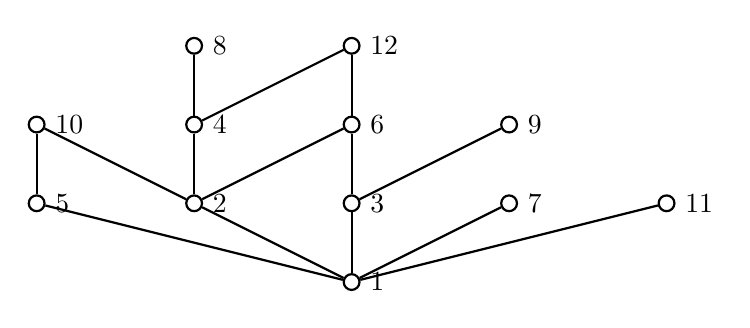
\begin{tikzpicture}[auto,
  specification/.style ={circle, draw, thick, inner sep = 0pt, minimum size=2mm}]
 \node[specification] (A)  [label=0:$1$] at (0,0)  {};
 \node[specification] (B)  [label=0:$5$] at (-4,1)  {};
 \node[specification] (C)  [label=0:$2$] at (-2,1)  {};
 \node[specification] (D) [label=0:$3$] at (0,1)  {};
 \node[specification] (E)  [label=0:$7$] at (2,1)  {};
 \node[specification] (F)  [label=0:$11$] at (4,1)  {};
 \node[specification] (G)  [label=0:$10$]at (-4,2)  {};
 \node[specification] (H)  [label=0:$4$] at (-2,2)  {};
 \node[specification] (I)  [label=0:$6$] at (0,2)  {};
 \node[specification] (J)  [label=0:$9$] at (2,2)  {};
 \node[specification] (K)  [label=0:$8$] at (-2,3)  {};
 \node[specification] (L)  [label=0:$12$] at (0,3)  {};
 \draw[thick] (A) to  (B);
 \draw[thick] (A) to  (C);
 \draw[thick] (A) to  (D);
 \draw[thick] (A) to  (E);
 \draw[thick] (A) to  (F);
 \draw[thick] (B) to  (G);
 \draw[thick] (C) to  (G);
 \draw[thick] (C) to  (H);
 \draw[thick] (C) to  (I);
 \draw[thick] (D) to  (I);
 \draw[thick] (D) to  (J);
 \draw[thick] (H) to  (K);
 \draw[thick] (H) to  (L);
 \draw[thick] (I) to  (L);
\end{tikzpicture}
  }

  极大元有$6$个:$7,8,9,10,11,12$

  极小元有$1$个:$1$
\end{proof}
\end{Exercise}
\end{CJK}
\end{document}


%%% Local Variables:
%%% mode: latex
%%% TeX-master: t
%%% End:
